\documentclass[12pt, twoside]{article}
\documentclass[12pt, twoside]{article}
\usepackage[letterpaper, margin=1in, headsep=0.2in]{geometry}
\setlength{\headheight}{0.6in}
%\usepackage[english]{babel}
\usepackage[utf8]{inputenc}
\usepackage{microtype}
\usepackage{amsmath}
\usepackage{amssymb}
%\usepackage{amsfonts}
\usepackage{siunitx} %units in math. eg 20\milli\meter
\usepackage{yhmath} % for arcs, overparenth command
\usepackage{tikz} %graphics
\usetikzlibrary{quotes, angles}
\usepackage{graphicx} %consider setting \graphicspath{{images/}}
\usepackage{parskip} %no paragraph indent
\usepackage{enumitem}
\usepackage{multicol}
\usepackage{venndiagram}

\usepackage{fancyhdr}
\pagestyle{fancy}
\fancyhf{}
\renewcommand{\headrulewidth}{0pt} % disable the underline of the header
\raggedbottom
\hfuzz=2mm %suppresses overfull box warnings

\usepackage{hyperref}
\usepackage{float}

\title{Algebra 2}
\author{Chris Huson}
\date{May 2024}

\fancyhead[LE]{\thepage}
\fancyhead[RO]{\thepage \\ Name: \hspace{1.5cm} \,\\}
\fancyhead[LO]{BECA/Huson/Algebra 2: Regents Preparation \\* 31 May 2024}

\begin{document}

\subsubsection*{Prep \#21: Normal distributions}
\begin{enumerate}[itemsep=0.5cm]
\item The mean intelligence quotient (IQ) score is 100, with a standard deviation of 15, and the scores are normally distributed. Given this information, find the approximate percentage of the population with an IQ greater than 130 to the \emph{nearest whole} percent. \vspace{3cm}

\item The distribution of the diameters of ball bearings made under a given manufacturing process is normally distributed with a mean of 4 cm and a standard deviation of 0.2 cm. What proportion of the ball bearings will have a diameter less than 3.7 cm?\vspace{4cm}

\item There are 440 students at Thomas Paine High School enrolled in U.S. History. On the April report card, the students' grades are approximately normally distributed with a mean of 79 and a standard deviation of 7. Students who earn a grade less than or equal to 64.9 must attend summer school. (sketch and label the distribution)  \begin{enumerate}
    \item Calculate the number of standard deviations the 64.9 cutoff score is from the mean. \vspace{1cm}
    \item What percentage of the students scored at or below 64.9? \vspace{2cm}
    \item Find the number of students who must attend summer school for U.S. History rounded to the \emph{nearest whole} student.
\end{enumerate} \vspace{2cm}


\newpage
\item Graph the function $f(x) = x^4-2x^{3}-5x^{2}+3x+4$. 
\begin{center}
    \begin{tikzpicture}[scale=0.65]
        \draw[lightgray,very thin] (-10,-10) grid (10,10);
        \draw [thick,<->] (-10.5,0)--(10.5,0) node [right] {$x$};
        \draw [thick,<->] (0,-10.5)--(0,10.5) node [above] {$f(x)$};
        \foreach \x in {2}
            \draw[thick] (\x cm,5pt) -- (\x cm,-5pt) node[below] {$1$};
        \foreach \y in {2}
            \draw[thick] (4pt,\y cm)--(-4pt,\y cm) node[left]{10};
    \end{tikzpicture}
    \end{center}
Mark and label the zeros of the function to the \emph{nearest hundredth}. \\[2cm]
Describe the behavior of the given function as $x$ approaches positive infinity.

\newpage
\item Convert between radical and rational exponent forms. (assume $x > 0$)
    \begin{multicols}{2}
    \begin{enumerate}
        \item $\displaystyle \frac{(9x)^{\frac{1}{2}} y}{y^{\frac{1}{2}}} =$
        \item $\displaystyle \frac{\sqrt[3]{8x^8}}{2 \sqrt{x^4}} = $
    \end{enumerate}
    \end{multicols} \vspace{2cm}

\item Explain what a rational exponent, such as $\frac{3}{2}$ means. Use this explanation to evaluate $\displaystyle 4^{\frac{3}{2}}$. \vspace{3cm}

\item Simplify each complex expression to the form $a+bi$.
    \begin{multicols}{2}
    \begin{enumerate}[itemsep=2cm]
        \item $i^2=$
        \item $(2-2i)(10+i)=$
        \item $(8+7i) - (5+3i)=$
        \item $\displaystyle \frac{1}{3} i (\sqrt{-81}+6i) + 5i=$

    \end{enumerate}
    \end{multicols} \vspace{3cm}

\newpage
\item Solve for $x$ over the complex numbers. \\[0.25cm]
$x^2-4x+13=0$
\vspace{5cm}

\item Solve algebraically for all values of $x$. \\[0.25cm]
$\sqrt{x+12}=x$ \vspace{5cm}

\item Solve algebraically for all values of $x$. \\[0.25cm]
$\displaystyle \frac{1}{x+12}=x$

\newpage
\item Write a recursive formula for the sequence 16, 8, 0, $-8$, $\ldots$ \vspace{2cm}

\item A sequence is defined by the recursive formula
\begin{align*}
a_1 &= 30 \\
a_{n} &= a_{n-1}+5
\end{align*}
Write an explicit formula for the sequence. \vspace{2cm}


\item The sum of the first $n$ terms of the geometric sequence beginning $1$, $1.5$, $2.25$, $\ldots$ is 171, rounded to \emph{the nearest integer}. Find $n$. \vspace{2cm}

%F.LE.2: Construct a linear or exponential function symbolically given: a graph, a description of the relationship, or two input-output pairs (including from a table).
\item Complete the table for the geometric sequence $a$.
    \begin{center}
    \begin{tabular}{|p{1cm}|p{1cm}|p{1cm}|p{1cm}|p{1cm}|p{1cm}|}
        \hline
        $n$ & 1 & 2 & 3 & 4 & 5 \\
        \hline
        $a_n$ & 100 & 80 & & & \\[0.25cm]
        \hline
    \end{tabular}
    \end{center}
    Model the sequence with an exponential function.


\newpage
\item A survey was conducted to compare the dietary habits of American and Japanese families. Families were asked which they had eaten for dinner most recently, meat or fish. The proportions of each answer are shown in the table below.
    \begin{center}
        \begin{tabular}{|c|c|c|c|}
            \hline
            Nationality & Meat & Fish & Total \\[0.2cm]
            \hline
            Americans & 0.78 & 0.22 & 1.00 \\[0.25cm]
            \hline
            Japanese & 0.43 & 0.57 & 1.00 \\[0.25cm]
            \hline
        \end{tabular}
    \end{center}
    \begin{enumerate}
        \item Does the survey data indicate that Americans and Japanese families have similiar dietary habits? Justify your answer. \vspace{2cm}
        \item 200 American families and 100 Japanese families participated in the survey. Calculate the number of each category of response and enter it in the appropriate cell in the table below. 
        \begin{center}
            \begin{tabular}{|c|p{1.5cm}|p{1.5cm}|c|}
                \hline
                Nationality & \; Meat & \; Fish & Total \\[0.2cm]
                \hline
                Americans & &  & 200 \\[0.25cm]
                \hline
                Japanese & &  & 100 \\[0.25cm]
                \hline
            \end{tabular}
        \end{center}
        \item The survey was conducted in Kansas City (an inland city) and Tokyo (a city on the Pacific Ocean). How might that affect the survey's findings? 
    \end{enumerate} \vspace{3cm}

\newpage
\item A manufacture of portable speakers finds that its profit varies depending on the number of speakers it makes. The profit, $p(x)$, in thousands of dollars as a function of the number of speakers, $x$, in thousands is modeled by $$p(x) = -x^3+7x^2+6x-25$$
\begin{enumerate}
    \item Graph $y=p(x)$, over the interval $0 \leq x \leq 8$ on the set of axes below.
    \item Over the given interval, state the coordinates of the maximum of $p$ rounding all values to the \emph{nearest integer}. Explain what the point means in terms of the number of speakers and profit. \vspace{3cm}
\end{enumerate}
\begin{center}
    \begin{tikzpicture}[yscale=0.1]
        \draw[gray,thin, xstep=1cm,ystep=10cm] (-3,-41) grid (10,80);
        \draw [thick,<->] (-3.5,0)--(10.5,0) node [right] {$x$};
        \draw [thick,<->] (0,-45)--(0,85) node [above] {$y$};
        \foreach \x in {1}
            \draw[thick] (\x cm,50pt) -- (\x cm,-50pt) node[below] {$\x$};
        \foreach \y in {20}
            \draw[thick] (4pt,\y cm)--(-4pt,\y cm) node[left]{$\y$};
        %\draw [thick,<->] plot[smooth, domain=-2.2:8] (\x, {-(\x*\x*\x)+7*(\x*\x)+6*(\x)-25});
    \end{tikzpicture}
    \end{center}

\newpage
\item Determine for which polynomial(s) $(x + 2)$ is a factor. Explain your answer.
 $$P(x) = x^4-3x^3-16x-12$$ 
 $$Q(x) = x^3-3x^2-16x-12$$ \vspace{10cm}

\item Given the function $P(x) = x^3-3x^2-2x+4$, find the value of $P(-1)$ and $P(1)$.\\[5cm]
Now identify the correct statement.
\begin{enumerate}
    \item $(x-1)$ is a factor because $P(-1)=2$.
    \item $(x+1)$ is a factor because $P(-1)=2$.
    \item $(x+1)$ is a factor because $P(1)=0$.
    \item $(x-1)$ is a factor because $P(1)=0$.
\end{enumerate}

\newpage

\item The data in the table was graphed and then a smooth curve was fit through the points. Write down an equation for the exponential function $f(x)$ shown.
    \begin{flushright}
    \begin{tabular}{|p{1cm}|p{1cm}|p{1cm}|p{1cm}|p{1cm}|p{1cm}|}
        \hline
        $n$ & 1 & 2 & 3 & 4 & 5 \\
        \hline
        $a_n$ & 100 & 80 & & & \\[0.25cm]
        \hline
    \end{tabular}
    \end{flushright}
    \begin{flushright}
    \begin{tikzpicture}[x=1cm, y=0.1cm, xscale=1.5]
        \draw [thin, color=lightgray, xstep=1cm,ystep=0.5cm] (0,0) grid (4,51);
        \draw [thick, ->] (0,0) -- (+4.3,0) node [below]{$x$};
        \draw [thick, ->] (0,0) -- (0,53) node [right]{$y$};        
        \foreach \x in {1}
            \draw (\x cm,5pt) -- (\x cm,-5pt) node[below] {$\x$};
        \foreach \y in {0,10,...,50}
            \draw[shift={(0,\y)}] (2pt,0pt)--(-2pt,0pt) node[left]{$\y$};
        \draw [thick, ->, smooth,domain=0.:4.2] plot(\x,{15*(3^(\x/4))});
        \fill (0,15) ellipse [x radius=1.33pt, y radius=2pt];
        \fill (4,45) ellipse [x radius=1.33pt, y radius=2pt];
    \end{tikzpicture}
    \end{flushright}

\item An investment of \$4000 earns a continuous interest rate of 8\%. On the axes below, graph the value of the investment $v(t)$ in thousands of dollars versus time $t$ in years. 
\begin{center}
    \begin{tikzpicture}[scale=0.8]
        \draw[gray,thin] (0,0) grid (10,10);
        \draw [thick,->] (0,0)--(10.5,0) node [right] {$t$};
        \draw [thick,->] (0,0)--(0,10.5) node [above] {$v(t)$};
        \foreach \x in {0,1,...,10}
            \draw (\x cm,5pt) -- (\x cm,-5pt) node[below] {$\x$};
        \foreach \y in {0,1,...,10}
            \draw[shift={(0,\y)}] (2pt,0pt)--(-2pt,0pt) node[left]{$\y$};
    \end{tikzpicture}
    \end{center}
Find the value of the investment after 5 years rounding to the \emph{nearest dollar}.

\newpage
\item Biologists are studying a new bacterium. They create a culture with 100 of the bacteria and
anticipate that the number of bacteria will double every 30 hours. Write an equation for the
number of bacteria, $B$, in terms of the number of hours, $t$, since the experiment began. %Jan 2020
\vspace{3cm}

\item During the summer, Adam saved \$4000 and Betty saved \$3500. Adam deposited his money in
Bank A at an annual rate of 2.4\% compounded monthly. Betty deposited her money in Bank B at
an annual rate of 4\% compounded quarterly. Write two functions that represent the value of each
account after $t$ years if no other deposits or withdrawals are made, where Adam's account value is represented by $A(t)$, and Betty's by $B(t)$. \vspace{5cm}
%Jan 2024

\item Solve algebraically for $x$ that makes the function value 125, to the \emph{nearest hundredth}, $f(x)=100 \times 10^{x}$. 

\end{enumerate}
\end{document}